%% LyX 2.1.4 created this file.  For more info, see http://www.lyx.org/.
%% Do not edit unless you really know what you are doing.
\documentclass[english]{article}
\usepackage[T1]{fontenc}
\usepackage[latin9]{inputenc}
\usepackage{geometry}
\geometry{verbose,tmargin=0.8in,bmargin=0.8in,lmargin=1in,rmargin=1in,headheight=0cm,headsep=0cm}
\usepackage{babel}
\usepackage{graphicx}
\usepackage[unicode=true]
 {hyperref}

\makeatletter

%%%%%%%%%%%%%%%%%%%%%%%%%%%%%% LyX specific LaTeX commands.
%% Because html converters don't know tabularnewline
\providecommand{\tabularnewline}{\\}

\makeatother

\begin{document}

\title{CSCE 221 Cover Page\\
 Homework Assignment \#3 \\
Due April 26 to CSNet}


\author{First Name~~Chris~~Last Name ~~~~~~~Comeaux~~~~~~UIN
622006681}


\date{User Name ~~~~~~~~cmc236~~~~~~~~~E-mail address~~~~~~~~~~~~~cmc236@tamu.edu~~~~~~~~~~~~~~\medskip{}
}
\maketitle
\begin{quotation}
\begin{flushleft}
Please list all sources in the table below including web pages which
you used to solve or implement the current homework. If you fail to
cite sources you can get a lower number of points or even zero, read
more Aggie Honor System Office \href{http://aggiehonor.tamu.edu/}{http://aggiehonor.tamu.edu/}\medskip{}
\medskip{}

\par\end{flushleft}
\end{quotation}
\begin{flushleft}
\begin{tabular}{|c|c|c|c|}
\hline 
Type of sources  & ~~~~~~~~~~~~~~~~~~~~~~~ & ~~~~~~~~~~~~~~~~~~~~~~~~ & ~~~~~~~~~~~~~~~~~~~~~~~\tabularnewline
 &  &  & \tabularnewline
\hline 
\hline 
People &  &  & \tabularnewline
 &  &  & \tabularnewline
\hline 
Web pages (provide URL)  & www.chegg.com &  & \tabularnewline
 &  &  & \tabularnewline
\hline 
Printed material & Data Structures and Algorithms &  & \tabularnewline
 & in c++ by Goodrich, Tamassia, and Mount &  & \tabularnewline
\hline 
Other Sources  &  &  & \tabularnewline
 &  &  & \tabularnewline
\hline 
\end{tabular}
\par\end{flushleft}


\date{\medskip{}
\medskip{}
}
\begin{quotation}
\begin{flushleft}
I certify that I have listed all the sources that I used to develop
the solutions/codes to the submitted work.
\par\end{flushleft}

\begin{flushleft}
\textquotedblleft On my honor as an Aggie, I have neither given nor
received any unauthorized help on this academic work.\textquotedblright{} 
\par\end{flushleft}
\end{quotation}

\date{\medskip{}
\medskip{}
}

\begin{flushleft}
\begin{tabular}{cccccc}
Your Name  & ~~~~~~~~~~~Chris~~~~~~~~~~~~~ &  & ~~~~~~~~~~Comeaux~~~~~~~~~~~ & Date  & ~~~~~~~~~4/25/2016~~~~~~~~~~~\tabularnewline
\end{tabular}\newpage{}
\par\end{flushleft}

\begin{flushleft}
\textbf{Homework 3}
\par\end{flushleft}

\begin{flushleft}
\textbf{due April 26 }
\par\end{flushleft}
\begin{enumerate}
\item \begin{flushleft}
(10 points) R-9.10 p. 417 
\par\end{flushleft}


\begin{flushleft}
What is the result of Exercise R-9.7, when collisions are handled
by double hashing using the secondary hash function $h_{s}(k)=7-(k$
mod 7)?$\newline$%
\begin{minipage}[t]{1\columnwidth}%
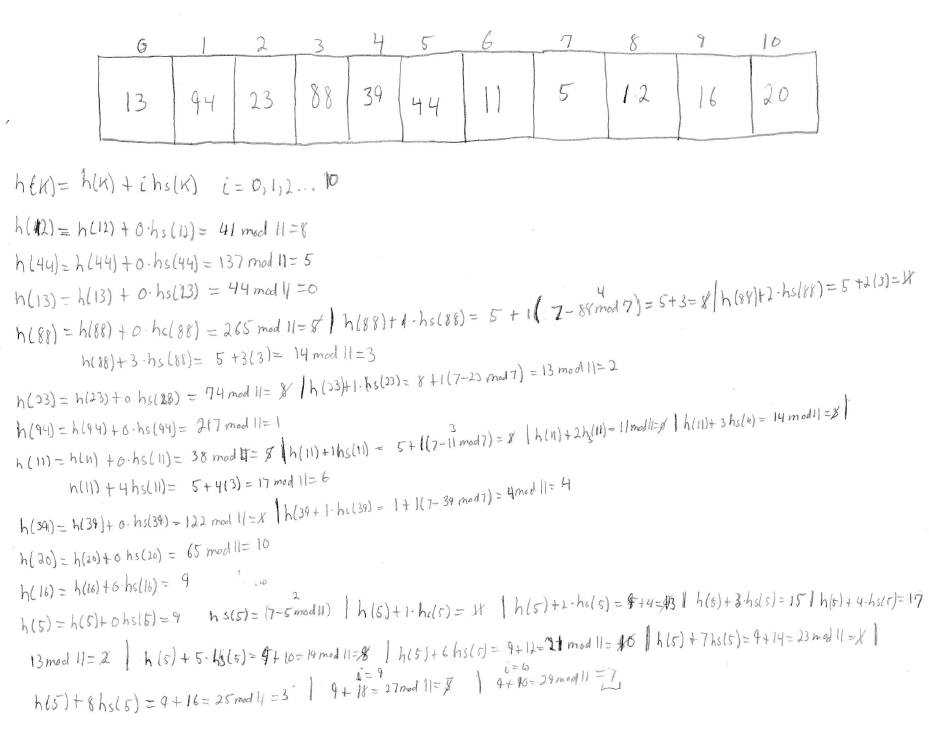
\includegraphics[scale=0.7]{1}%
\end{minipage}
\par\end{flushleft}

\item \begin{flushleft}
(10 points) R-8.2 p. 361
\par\end{flushleft}


\begin{flushleft}
How long would it take toremove $\left\lceil log\,n\right\rceil $
smallest elements from a heap that contains $n$ entries using the
\texttt{removeMin()} operation?$\newline$$\newline$%
\begin{minipage}[t]{1\columnwidth}%
\begin{flushleft}
The remiveMin function takes $log_{2}n$. For a heap with n elements,
to remove the smallest $log\,n$ elements, with the removeMin function
it would take $O(log_{2}(log_{2}n)).$
\par\end{flushleft}%
\end{minipage}\newpage{}
\par\end{flushleft}

\item \begin{flushleft}
(10 points) R-8.7 p. 361
\par\end{flushleft}


\begin{flushleft}
An airport is developing a computer simulation of air-traffic control
that handles events such as landings and takeoffs. Each event has
a \emph{time-stamp }that denotes the time when the event occurs. The
simulation program needs to efficiently perform the following two
fundamental operations:
\par\end{flushleft}
\begin{itemize}
\item \begin{flushleft}
Insert an event with a given time-stamp (that is, add a future event)
\par\end{flushleft}
\item \begin{flushleft}
Extract the event with smallest time-stamp (that is, determine the
next event to process)
\par\end{flushleft}
\end{itemize}

\begin{flushleft}
Which data structure should be used for the above operations? Why?$\newline$%
\begin{minipage}[t]{1\columnwidth}%
\begin{flushleft}
A priority queue implemented with a binary hap would be best because
it can insert and extract in logarithmic time. Even though an unsorted
array can insert in constant time, it take linear time to removeMin.
Likewise, a sorted array can removeMin in constant time but is takes
linear time to insert a new event.
\par\end{flushleft}%
\end{minipage}
\par\end{flushleft}

\item \begin{flushleft}
(10 points) R-13-3 and R-13-4, p. 654 %
\begin{minipage}[t]{1\columnwidth}%
\begin{flushleft}
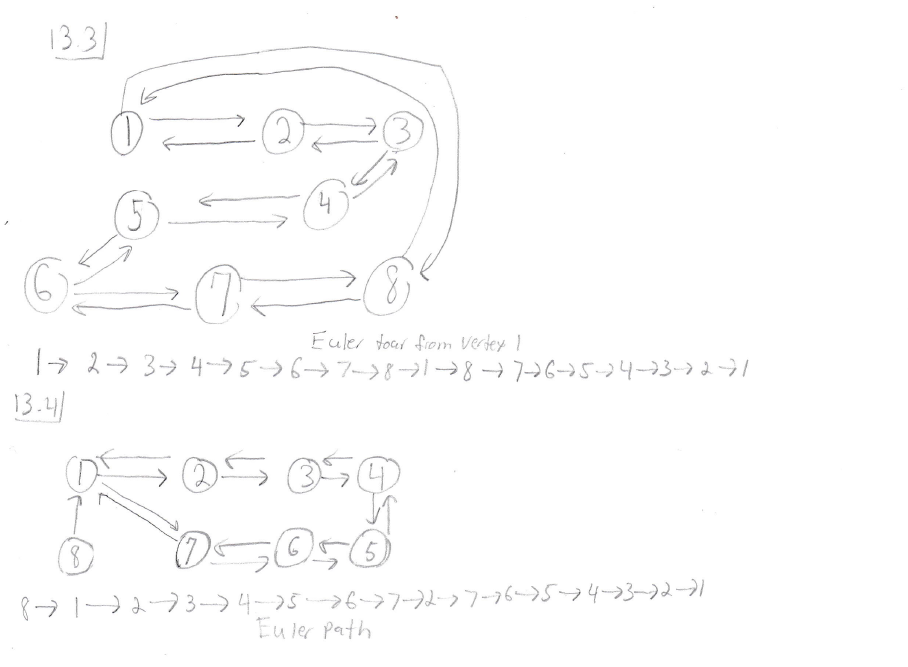
\includegraphics[scale=0.75]{4}
\par\end{flushleft}%
\end{minipage}\newpage{}
\par\end{flushleft}
\item \begin{flushleft}
(10 points) R-13.8, p. 655$\newline$%
\begin{minipage}[t]{1\columnwidth}%
\begin{flushleft}
\textbf{A. Adjacency list. }This is because it would take $10^{8}(10,000*10,000)$
Boolean bits to represent the graph as a adjacency matrix. It would
take less space to use an adjacency list (enough to hold 20,000 nodes).
\par\end{flushleft}

\textbf{B. Adjacency Matrix. }The adjacency matrix would take around
$4*10^{14}$ bits which is a lot. However, the adjacency list would
have to store 20,000,000 edges. Depending on how large each node is
in the list, the space being used can grow very fast with that amount
of nodes.$\newline$

\textbf{C. Adjacency Matrix.} Since space is not a factor, adjacency
matrix would be the best choice because it can evaluate isAdjecentTo
in constant time. On the other hand, the adjacency list would have
to iterate through each edge adjacent to that vertex. %
\end{minipage}
\par\end{flushleft}
\item \begin{flushleft}
(10 points) R-13.16, p. 656$\newline$%
\begin{minipage}[t]{1\columnwidth}%
\begin{flushleft}
\textbf{Algorithm }ShortestPath(G,v)
\par\end{flushleft}

Initialize D{[}v{]}=0 and D{[}u{]} = positive infinity for all u !=
v. 

Priority Queue Que; //contains all vertices of the Graoh G using key
as the labels

while(!Queue.empty())

\{

$\indent$u=Que.removeMin() //pull u into cloud

for each vertex z adjacent to u that has not been visited

\{

$\indent$Update D{[}z{]} and display its distance and path

$\indent$if(D{[}z{]} > D{[}u{]} + w(u,z) )// relax function

$\indent$\{

$\indent$$\indent$D{[}z{]} = D{[}u{]} + w(u,z) 

$\indent$$\indent$P{[}z{]} = u

$\indent$\}

$\indent$cout<\textcompwordmark{}<''Distance from `` <\textcompwordmark{}<v
<\textcompwordmark{}<''to'' <\textcompwordmark{}<u <\textcompwordmark{}<''is''
<\textcompwordmark{}<D{[}z{]}

$\indent$cout<\textcompwordmark{}<''Path from `` <\textcompwordmark{}<v
<\textcompwordmark{}<''to'' <\textcompwordmark{}<u <\textcompwordmark{}<''is
v ->'' <\textcompwordmark{}<z <\textcompwordmark{}<''->u''

\}

\}%
\end{minipage}
\par\end{flushleft}
\item \begin{flushleft}
(10 points) R-13.17, p. 656$\newline$$\newline$%
\begin{minipage}[t]{1\columnwidth}%
\begin{flushleft}
3->5 (115); 1->8( 120); 2->8 (155); 4->5 (160); 5->8 (170); 2->6 (180)
\par\end{flushleft}%
\end{minipage}\newpage{}
\par\end{flushleft}
\item \begin{flushleft}
(10 points) You want to help CS/CSE freshman students to prepare their
course schedules for the first two years in the lower level division.
By building a directed graph suggest order in which they should schedule
their courses taking into account their corresponding prerequisites.
A set of vertices represents courses and a set of edges represents
a dependence of a given course on a course prerequisite.$\newline$
\begin{minipage}[t]{1\columnwidth}%
\begin{flushleft}
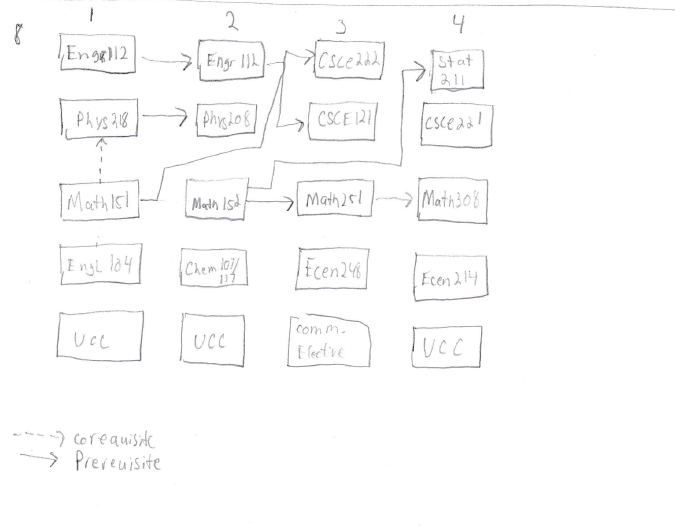
\includegraphics[scale=0.75]{8}
\par\end{flushleft}%
\end{minipage}
\par\end{flushleft}
\item \begin{flushleft}
(10 points) R-13.31, p. 656$\newline$%
\begin{minipage}[t]{1\columnwidth}%
\begin{flushleft}
A tree that contains all vertices in the graph in a straight line.
In other words, every node, besides the last node, has exactly one
child, and every node, besides the root, has exactly one parent. Like
this: a->b->c->d->...->z
\par\end{flushleft}%
\end{minipage}
\par\end{flushleft}
\item \begin{flushleft}
(10 points) Write what the running time, and provide its justification,
of the Dijkstra's algorithm is for a sparse and dense graph and the
priority queue implemented based on
\par\end{flushleft}

\begin{enumerate}
\item \begin{flushleft}
a binary heap
\par\end{flushleft}
\item \begin{flushleft}
an unsorted list
\par\end{flushleft}
\item \begin{flushleft}
a sorted list$\newline$%
\begin{minipage}[t]{1\columnwidth}%
\begin{flushleft}
Dijkstra's algorithm: $O(n*removeMin())$$+$$(m*DecreaseKey())$
Sparce = n=m. Dense=$n^{2}=m$.
\par\end{flushleft}

A. Binary Heap: removeMin = $O(log_{2}n)$, DecreaseKey = $O(n)$
-> $O(nlog_{2}n)+(m*n)$.

Sparse graph: $O(nlog_{2}n)+(n^{2})$= $O(n^{2})$ without locators
and $O(nlog_{2}n)$ with locators.

Dense graph: $O(nlog_{2}n)+(n^{3})$ = $O(n^{3})$ without locators
and $O(n^{2}log_{2}n)$ with locators$\newline$

B. Unsorted Graph: removeMin = $O(n)$ and DecreaseKey = $O(n)$ ->
$O(n*n)+(m*n).$

Sparse graph: $O(n^{2})+(n^{2})$ = $O(n^{2})$.

Dense graph: $O(n^{2})+(n^{3})$ = $O(n^{3})$$\newline$

C. Sorted Graph: removeMin = $O(1)$ and DecreaseKey = $O(n)$ ->
$O(n+m*n).$

Sparse graph: $O(n+n^{2})$ = $O(n^{2})$.

Dense graph: $O(n+n^{3})$ = $O(n^{3})$%
\end{minipage}
\par\end{flushleft}
\end{enumerate}
\item \begin{flushleft}
(10 points) C-13.10, p. 658$\newline$%
\begin{minipage}[t]{1\columnwidth}%
\begin{flushleft}
For an Euler tour, every vertex needs two sets of edges. Two edges
that com out from the previous and next vertex in the tour and two
edges that does in the previous and next vertex in the tour. This
means the each vertex has two edges going in and out of it. Therefore,
the number of edges is 2 times the number of nodes meaning m=2n. So,
$O(n+m)$ = $O(n+2n)=O(3n)=O(n)$.
\par\end{flushleft}%
\end{minipage}
\par\end{flushleft}
\item \begin{flushleft}
(10 points) C-13.15, p. 659$\newline$%
\begin{minipage}[t]{1\columnwidth}%
\begin{flushleft}
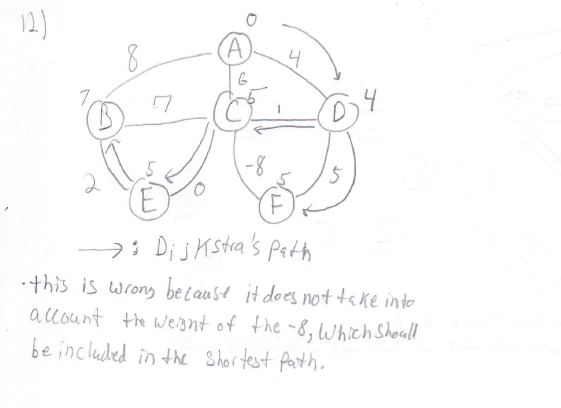
\includegraphics[scale=0.75]{12}
\par\end{flushleft}%
\end{minipage}
\par\end{flushleft}
\item \begin{flushleft}
(10 points) C-13.18, p. 659$\newline$%
\begin{minipage}[t]{1\columnwidth}%
\begin{flushleft}
Using Dijkstra's algorithm we can change the Relax function from if(D{[}z{]}
> D{[}u{]} + w(u,z) ) to if(D{[}z{]} < D{[}u{]} + w(u,z) ). This will
find the longest path instead of the shortest. The running time based
on the implementation with a priority queue using a binary heap and
locators would be $O(nlog_{2}n)$ and $O(n^{2})$ without locators. 
\par\end{flushleft}

\begin{flushleft}
\textbf{Algorithm }LongestPath(G,v)
\par\end{flushleft}

Initialize D{[}v{]}=0 and D{[}u{]} = positive infinity for all u !=
v. 

Priority Queue Que; //contains all vertices of the Graph G using key
as the labels

while(!Queue.empty())

\{

$\indent$u=Que.removeMin() //pull u into cloud

for each vetex z adjencent to u that has not been visited

\{

$\indent$if(D{[}z{]} < D{[}u{]} + w(u,z) )// relax function

$\indent$\{

$\indent$$\indent$D{[}z{]} = D{[}u{]} + w(u,z) 

$\indent$$\indent$P{[}z{]} = u

$\indent$\}

\}

\}%
\end{minipage}
\par\end{flushleft}\end{enumerate}

\end{document}
